%Data da última atualização: 04/11/2016

\chapter{Problemas para o 6º ano}
\section{As Quatro Operações}
\subsection{Adição}

\begin{list}{\textbf{Questão \arabic{quest}.}}{\usecounter{quest}}
%define a margem da lista.	
%\setlength{\labelwidth}{-2mm} \setlength{\parsep}{0mm}
%\setlength{\topsep}{0mm} \setlength{\leftmargin}{-2mm}
\renewcommand{\labelenumi}{(\alph{enumi})}

\item Calcule as somas
\begin{multicols}{4}
\begin{enumerate}[a)]
	\item 10 + 11 = 21
	\item 10 + 21 = 31
	\item 10 + 31 = 41
	\item 10 + 41 = 51
	\item 10 + 51 = 61
	\item 10 + 61 = 71
	\item 10 + 71 = 81
	\item 10 + 81 = 91
	\item 10 + 91 = 101
	\item 12 + 66 = 78
	\item 13 + 48 = 61
	\item 67 + 89 = 156
	\item 97 + 89 = 186
	\item 56 + 87 = 143
	\item 84 + 77 = 161
	\item 38 + 98 = 136
	\item 69 + 73 = 142
	\item 83 + 99 = 182
	\item 73 + 37 = 110
	\item 75 + 23 = 98
	\item 37 + 67 = 104
	\item 88 + 88 = 176
	\item 99 + 99 = 198
\end{enumerate}
\end{multicols}

\item calcule as somas

\begin{multicols}{4}
\begin{enumerate}[a)]
	\item 110 + 100 
	\item 120 + 101 
	\item 130 + 111 
	\item 140 + 121 
	\item 150 + 131 
	\item 170 + 132 
	\item 180 + 134 
	\item 190 + 135 
	\item 200 + 136
	\item 201 + 137 
	\item 210 + 138 
	\item 220 + 139
	\item 230 + 140 
	\item 240 + 150 
	\item 250 + 160 
	\item 260 + 170 
	\item 270 + 180
	\item 280 + 190
	\item 290 + 200
	\item 311 + 212
	\item 548 + 645
	\item 665 + 912
	\item 987 + 789
\end{enumerate}
\end{multicols}

\item Efetue as adições

\begin{multicols}{4}
\begin{enumerate}[a)]
	\item 1487 + 2365
	\item 6547 + 5478
	\item 4589 + 4587
	\item 3258 + 9632
	\item 7896 + 5697
	\item 5423 + 8912
	\item 7463 + 9641
	\item 2536 + 5847
	\item 7788 + 9988
	\item 1122 + 4477
	\item 7946 + 3146
	\item 4562 + 3215
	\item 1478 + 8632
	\item 8437 + 2791
	\item 2491 + 8461
	\item 6258 + 6412
	\item 5353 + 7887
	\item 3226 + 9558
	\item 1112 + 9994
	\item 6537 + 4538
	\item 2197 + 8617
	\item 1002 + 9913
	\item 9999 + 8888
\end{enumerate}
\end{multicols}

\item Efetue as adições

\begin{multicols}{2}
\begin{enumerate}[a)]
	\item 296 + 1634 + 98
	\item 109 + 432 + 7482
	\item 48 + 16409 + 287
	\item 31 + 1487 + 641 + 109
	\item 3412 + 1246
\end{enumerate}
\end{multicols}

\item Determine a soma do número 273 com o seu sucessor

\item Um objeto custa R\$ 415.720,00. O comprador terá ainda R\$ 28.912,00 de despesa de frete. Quanto o comprador vai pagar?

\item Ao receber o meu salário paguei R\$ 437,12 de aluguel, R\$ 68,14 de impostos, R\$ 1.089,67 de gastos com alimentação e ainda me sobraram R\$ 749,18. Quanto recebi de salário?

\item Um menino estuda 2 horas e 45 minutos pela manhã e 4 horas e 30 minutos à tarde. Quantos minutos estuda diariamente?

\item Um automóvel passou pelo quilômetro 435 de uma rodovia. Ele ainda deverá percorrer 298 quilômetros até chegar ao seu destino. Quantos quilômetros da estrada vai percorrer para chegar ao destino?

\item Em 1990 o Brasil vendeu para o exterior 283.356 veículos e, em 1991, essa venda foi de 345.760 veículos. Quantos veículos o Brasil vendeu para o exterior nesses dois anos?

\item Uma empresa tem sede em São Paulo e filiais em outros estados. Na sede trabalham 316 pessoas e nas filiais 1098 pessoas. Quantas pessoas trabalham nessa empresa?

\item Em um condomínio, há 675 lotes já vendidos e 1095 lotes para vender. Quantos lotes de terreno há nesse condomínio?

\item Uma escola funciona em dois turnos. No turno matutino há 1407 alunos e no turno vespertino há 1825 alunos. Quantos alunos estudam nessa escola?

\item Uma empresa produziu no primeiro trimestre 6905 peças. no segundo trimestre, a mesma empresa produziu 795 peças a mais que no primeiro trimestre. Nessas condições:
\begin{enumerate}
	\item Quantas peças a empresa produziu no segundo trimestre?
	\item Quantas peças a empresa produziu no semestre?
\end{enumerate}

\item Nei comprou um aparelho de som por 635 reais e as caixas de som por 128 reais. Tendo pago 12 reais pela instalação, qual a quantia que ele gastou ?

\item De acordo com o censo realizado em 1991, o estado da Paraíba tem 1.546.042 homens e 1.654.578 mulheres. Qual é a população da Paraíba segundo esse censo?

\item Calcule:

\begin{multicols}{3}
\begin{enumerate}[a)]
	\item 1705 + 395 
	\item 11.048 + 9.881 
	\item 4.907 + 62.103 
	\item 275.103 + 94.924 
	\item $545 + 2.298 + 99$
	\item $7.502 + 209.169 + 38.425$
\end{enumerate}
\end{multicols}

\end{list}

\subsection{Subtração}
\begin{list}{\textbf{Questão \arabic{quest}.}}{\usecounter{quest}}
%define a margem da lista.	
%\setlength{\labelwidth}{-2mm} \setlength{\parsep}{0mm}
%\setlength{\topsep}{0mm} \setlength{\leftmargin}{-2mm}
\renewcommand{\labelenumi}{(\alph{enumi})}

\item Calcule as subtrações
\begin{multicols}{3}
\begin{enumerate}[a)]
	\item 47 - 31
	\item 58 - 45
	\item 65 - 57
	\item 89 - 65
	\item 97 - 21
	\item 78 - 34
	\item 56 - 31
	\item 87 - 78
	\item 98 - 78
	\item 48 - 29
	\item 38 - 29
	\item 68 - 59
	\item 56 - 37
	\item 23 - 19
	\item 99 - 81
	\item 21 - 19
	\item 23 - 22
	\item 18 - 14
	\item 74 - 49
	\item 74 - 37
	\item 74 - 52
	\item 74 - 63
	\item 96 - 13
	 
\end{enumerate}
\end{multicols}

\item Calcule as Subtrações
\begin{multicols}{3}
\begin{enumerate}[a)]
	\item 72224 - 6458
	\item 701 - 638
	\item 131003 - 88043
	\item 1138 - 909
	\item 80469 - 6458
	\item 866 - 638
	\item 131012 - 88142
	\item 2238 - 909
	\item 802 - 638
\end{enumerate}
\end{multicols}

\item Dom Pedro II, imperador do Brasil, faleceu em 1891 com 66 anos de idade. Em que ano ele nasceu?

\item Um avião Boeing 747 pode transportar 370 passageiros e um avião DC-10 pode transportar 285 passageiros. Quantos passageiros o Boeing 747 pode transportar a mais que o DC-10?

\item À vista um automóvel custa 26.454 reais. À prazo o mesmo automóvel custa 38.392 reais. A diferença entre o preço cobrado é chamado de juros. Qual é a quantia que pagará de juros?

\item Um avião pode transportar 295 passageiros. Em determinado vôo, o avião está transportando 209 passageiros. Quantas poltronas desse avião não estão ocupadas?

\item Se Antônio tem 518 selos e Pedro tem 702 selos, Quantos selos Pedro tem a mais que Antônio?

\item Ézio tem 95 reais e quer comprar uma máquina fotográfica que custa 130 reais. Quantos reais faltam para ele comprar a máquina?

\item De acordo com o Censo de 1980, a população de uma cidade era de 79.412 habitantes. Feito o Censo em 1991, verificou-se que a população dessa cidade passou a ser de 94.070 habitantes. Qual foi o aumento da população dessa cidade nesse período de tempo?

\item Uma industria, no final de 1991, tinha 10.635 empregados. No inicio de 1992 em virtude da crise econômica dispensou 1.880 funcionários. Com quantos funcionários a indústria ficou?

\item Qual a diferença entre 10.000 e 5.995?

\item Quantas unidades faltam a 499 para atingir 1 unidade de milhar?

\item Efetue:
\begin{multicols}{4}
\begin{enumerate}[a)]
	\item 2620 - 945
	\item 7000 - 1096
	\item 11011 - 7997
	\item 140926 - 78016
\end{enumerate}
\end{multicols}

\item Considere os números 645 e 335. Nessas condições:
\begin{enumerate}[a)]
	\item Determine a diferença entre eles
	\item Adicione 5 unidades ao primeiro número e 5 unidades ao segundo número e calcule a diferença entre os novos números que você obteve. 
\end{enumerate}

\end{list}

\subsection{Multiplicação}

\begin{list}{\textbf{Questão \arabic{quest}.}}{\usecounter{quest}}
%define a margem da lista.	
%\setlength{\labelwidth}{-2mm} \setlength{\parsep}{0mm}
%\setlength{\topsep}{0mm} \setlength{\leftmargin}{-2mm}
\renewcommand{\labelenumi}{(\alph{enumi})}


\item Calcule as multiplicações
\begin{multicols}{4}
\begin{enumerate}[a)]
	\item 5 x 5 =
	\item 5 x 15
	\item 5 x 115
	\item 5 x 25 =
	\item 5 X 125 =
	\item 5 x 55 =
	\item 5 x 75 =
	\item 5 x 375 =
	\item 5 x 1257 =
	\item 6 x 5 =
	\item 6 x 15 = 
	\item 6 x 115 =
	\item 6 x 25 =
	\item 6 x 125 =
	\item 6 x 55 =
	\item 6 x 75 =
	\item 6 x 375 =
	\item 6 x 1257 =
	\item 7 x 5 =
	\item 7 x 15 =
	\item 7 x 115 =
	\item 7 x 25 =
	\item 7 x 125 =
	\item 7 x 55 =
\end{enumerate}
\end{multicols}

\item Calcule as multiplicações
\begin{multicols}{3}
\begin{enumerate}[a)]
	\item 7 x 75 =
	\item 7 x 375 =
	\item 7 x 1257 =
	\item 8 x 5 =
	\item 8 x 15 = 
	\item 8 x 115 =
	\item 8 x 25 =
	\item 8 x 125 =
	\item 8 x 55 =
	\item 8 x 75 =
	\item 8 x 375 =
	\item 8 x 1257 =
	\item 9 x 5 =
	\item 9 x 15 =
	\item 9 x 115 =
	\item 9 x 25 =
	\item 9 x 125 =
	\item 9 x 55 =
	\item 9 x 75 =
	\item 9 x 375 =
	\item 9 x 1257 =
	\item 9 x 999 =
	\item 9 x 123 =
\end{enumerate}
\end{multicols}

\item Efetue as Multiplicações
\begin{multicols}{3}
\begin{enumerate}[a)]
	\item 153 x 7 =
	\item 1007 x 9 =
	\item 509 x 62 =
	\item 758 x 46 =
	\item 445 x 93 =
	\item 289 x 140 =
	\item 1782 x 240 =
	\item 2008 x 405 =
	\item 2453 x 1002 =
\end{enumerate}
\end{multicols}

\item Efetue as multiplicações
\begin{multicols}{3}
\begin{enumerate}[a)]
	\item 28 x 0 =
	\item 49 x 10 =
	\item 274 x 10 =
	\item 158 x 100 =
	\item 164 x 1000 =
	\item 89 x 10000 =
\end{enumerate}
\end{multicols}

\item  Considerando 1 mês = 30 dias e 1 ano = 365 dias, uma semana = 7 dias, determine:
\begin{enumerate}[a)]
	\item quantos dias há em 15 semanas completas.
	\item Quantos dias há em 72 meses completos.
	\item Quantos dias há em 8 anos completos.
\end{enumerate}  

\item Para uma demonstração de ginástica, um professor de Educação Física prepara 64 grupos de alunos. Cada grupo é formado por 25 alunos. Quantos alunos devem participar dessa demostração?

\item Com 12 prestações mensais iguais de 325 reais posso comprar uma moto. Quanto vou pagar por essa moto? R: 3900 reais

\item Qual é o número natural que você vai obter quando multiplicar 736 por 208?

\item  Para cobrir o piso de um barracão foram colocados 352 placas de 35 metros quadrados cada uma. Quantos metros quadrados tem o piso desse barracão?

\item Um carro bem regulado percorre 12 quilômetros com um litro de gasolina. Se numa viagem foram consumidos 46 litros, qual a distância em quilômetros que o carro percorreu? 

\item Em um teatro há 18 fileiras de poltronas. Em cada fileira foram colocadas 26 poltronas. Quantas poltronas há nesse teatro? 
.
\item Em uma multiplicação, os fatores são 134 e 296. Qual o produto?

\item Numa mercearia há 7 caixas de bombons e cada caixa contém 3 duzias de bombons. Quantos bombons há na mercearia? 

\item Uma pessoa deu R\$ 4.700,00 de entrada na compra de um objeto e pagou mais 6 prestações de R\$ 2.300,00. Quanto custou o objeto?

\item Um motorista percorreu 749 km em 6 dias. Nos cinco primeiros dias andou 132 km por dia. Quanto percorreu no 6º dia ?

\item Calcule:
\begin{multicols}{3}
\begin{enumerate}[a)]
	\item 19 x 6 =
	\item 46 x 12 =
	\item 321 x 11 =
	\item 329 x 25 =
	\item 1246 x 24 =
	\item 67632 x 101 =
\end{enumerate}
\end{multicols}

\item Calcule as contas:
\begin{multicols}{3}
\begin{enumerate}[a)]
	\item 18 x 5 x 2 =
	\item 5 x 2 x 24 =
	\item 2 x 5 x 44 =
	\item 37 x 2 x 5 =
	\item 12 x 4 x 5 =
	\item 4 x 5 x 15=
\end{enumerate}
\end{multicols}

\item Em um banheiro tem uma parede com 15 fileiras com 10 azulejos e outra parede com 13 fileiras com 10. Quantos azulejos têm no banheiro? 

\item  Qual é o resultado da multiplicação de 63 por 12? 

\end{list}

\subsection{Divisão}

\begin{list}{\textbf{Questão \arabic{quest}.}}{\usecounter{quest}}
%define a margem da lista.	
%\setlength{\labelwidth}{-2mm} \setlength{\parsep}{0mm}
%\setlength{\topsep}{0mm} \setlength{\leftmargin}{-2mm}
\renewcommand{\labelenumi}{(\alph{enumi})}

\item Calcule as divisões
\begin{multicols}{3}
\begin{enumerate}[a)]
	\item 20:5=
	\item 16:8=
	\item 12:1=
	\item 48:8=
	\item 37:37=
	\item 56:14=
\end{enumerate}
\end{multicols}

\item Observe a igualdade $56\div 7=8$ e responda:
\begin{multicols}{2}
\begin{enumerate}[a)]
	\item Qual é o nome da operação?
	\item Como se chama o número 56?
	\item Como se chama o número 7?
	\item como se chama o número 8?
\end{enumerate}
\end{multicols}

\item Efetue as divisões
\begin{multicols}{3}
\begin{enumerate}[a)]
	\item 492:4= 
	\item 91:9=
	\item 4416:6=
	\item 2397:17=
	\item 1584:99=
	\item 1442:14=
	\item 21000:15=
	\item 7650:102=
	\item 11376:237=
\end{enumerate}
\end{multicols}

\item Responda
\begin{multicols}{2}
\begin{enumerate}[a)]
	\item Qual é a metade de 784?
	\item Qual é a terça parte de 144?
	\item Qual é a quinta parte de 1800?
	\item Qual é a décima parte de 3500?
\end{enumerate}
\end{multicols}

\item Em um teatro há 126 poltronas distribuídas igualmente em 9 fileiras. Quantas poltronas foram colocadas em cada fileira?

\item Quantos garrafões de 5 litros são necessários para engarrafar 315 litros de vinho?

\item Uma pessoa ganha R\$ 23,00 por hora de trabalho. Quanto tempo deverá trabalhar para receber R\$ 391,00?

\item Uma torneira despeja 75 litros de água por hora. Quanto tempo levará para encher uma caixa de 3150 litros ?

\item Numa pista de atletismo uma volta tem 400 metros. Numa corrida de 10.000 metros, quantas voltas o atleta tem de dar nessa pista?

\item Um livro tem 216 páginas. Quero terminar a leitura desse livro em 18 dias, lendo o mesmo número de páginas todos os dias. Quantas páginas preciso ler por dia?

\item Quantos grupos de 18 alunos podem ser formados com 666 alunos?

\item Uma tonelada de cana de açúcar produz aproximadamente 85 litros de álcool. Quantas toneladas de cana são necessárias para produzir 6970 litros de álcool?

\item Determine o quociente e o resto das seguintes divisões:
\begin{multicols}{3}
\begin{enumerate}[a)]
	\item 79:8= 
	\item 49:8= 
	\item 57:8= 
	\item 181:15= 
	\item 3214:10= 
	\item 825:18= 
	\item 4937:32= 
	\item 7902:12=
	\item 1545:114=
\end{enumerate}
\end{multicols}

\end{list}

\section{Problemas Envolvendo Adição e Subtração}
\begin{list}{\textbf{Questão \arabic{quest}.}}{\usecounter{quest}}
%define a margem da lista.	
%\setlength{\labelwidth}{-2mm} \setlength{\parsep}{0mm}
%\setlength{\topsep}{0mm} \setlength{\leftmargin}{-2mm}
\renewcommand{\labelenumi}{(\alph{enumi})}

	\item Resolva os problemas registrando todos os cálculos e a resposta de forma clara e completa.
	\begin{enumerate}[a)]
		\item Em uma escola de 612 alunos, 325 foram vacinados contra a gripe. Quantos alunos ainda precisam tomar a vacina? 
		\item Uma empresa de reciclagem de alumínio troca 1250 latas por um computador. A escola de Iara já juntou 763 latinhas. Quantas latinhas faltam para a escola de Iara ter a quantidade necessária para receber o computador?
		\item A diretora de uma escola organizou uma campanha de doação de livros para melhorar a biblioteca. Conseguiram 347 livros de doação e agora a biblioteca conta com 958 exemplares. Quantos livros a biblioteca tinha antes da campanha?
		\item José ficou muito confuso depois de bater figurinhas com Miguel. Tinham jogado duas partidas. José lembrava que na primeira partida ganhou 45 figurinhas e na segunda perdeu 52 figurinhas.Agora contava várias vezes as 63 figurinhas que ficaram em sua mão, sem se dar conta de quantas tinha antes de começar a jogar. Quantas figurinhas tinha José ao começar o jogo?
		\item No álbum de Ricardo cabem 356 figurinhas. Ele já colou 119. Quantas figurinhas Ricardo precisa colar para completar seu álbum?
		\item Mariana coleciona adesivos. No seu aniversário, ganhou 15 adesivos de seu avô e 6 de seu irmão. Como tinha alguns repetidos, deu 20 de presente a uma amiga que também coleciona adesivos, Como ficou a coleção de adesivos de Mariana? Ela ficou com mais ou com menos adesivos do que antes de seu aniversário: Quantos a mais ou quantos a menos?
		\item Hélio fez uma viagem de caminhão e abasteceu o tanque duas vezes, colocando 135 litros em cada parada. Durante toda a viagem consumiu 258 litros. Sobrou combustível no final da viagem? Justifique sua resposta.
		\item Embarcaram em um trem 420 pessoas na primeira estação. Na segunda estação subiram mais 130 pessoas e desceram 360. Na parada seguinte, desceram 340 pessoas e subiram 210. Quantas pessoas ficaram no trem após essas paradas?
		\item Um fazendeiro possui 524 bois. Na feira de gado vendeu 183 de seus bois e comprou outros 266 bois. Quantos bois o fazendeiro tem agora?
		\item Ana deve 315 reais para Paula e Paula deve 238 reais para Ana. Quem deve pagar a quem para saldar as dívidas? Quanto?
		\item Estou poupando para comprar uma bicicleta de R\$ 300,00. Minha mãe me deu R\$ 130,00, meu padrinho me presenteou com R\$ 82,00 e meu irmão mais velho me deu R\$ 25,00 em uma semana e R\$ 17,00 na outra . O que eu juntei dá para comprar a bicicleta? Sobra o falta? Quanto?
		\item Lucas nasceu em 1984. Quantos anos completará em 2020?		
	\end{enumerate}
	
	\item Sete amigos querem repartir 630 reais entre eles. Todos têm que receber a mesma quantia e não pode sobrar nada. Como podem fazer a divisão? Quanto cabe a cada um?
	\item A avó de Paula repartiu 56 reais igualmente entre seus netos de tal maneira que cada um recebeu 8 reais. Entre quantos netos ele repartiu o dinheiro?
	\item A professora do 5º ano repartiu 90 lápis de cor entre alguns alunos. Cada aluno recebeu 9 lápis. Quantos alunos receberam lápis de cor?
	\item Aílton quer plantar, em sua chácara, 45 limoeiros em 5 filas. Quantos limoeiros deve plantar em cada fileira?
	\item Uma padaria prepara 140 tortas todos dos dias. Para assá-las o padeiro coloca 8 tortas em cada bandeja. Quantas bandejas são necessárias para assar todas as tortas?
	
	\item Em uma campanha de vacinação a previsão era de que no mínimo 20 000 crianças fossem vacinadas em dois dias. No primeiro dia foram vacinadas 11 640 crianças e no segundo dia, 3 264 crianças a menos do que no dia anterior. Verifique se o objetivo foi alcançado.
	\item Na escola de Pedro há 8 classes de 35 alunos, 5 classes de 33 alunos e 12 classes de  30 alunos. Qual o total de alunos nessa escola?
	\item Fabrício tinha 320 reais para pagar as contas (117 reais de energia elétrica, 58 reais de água e 88 reais de telefone) e para fazer algumas compras. Quanto lhe restou para fazer as compras?
	\item Foram repartidas 45 balas entre três crianças: Raul e Mara receberam quantidades iguais e Paula recebeu 3 balas a mais do que Raul. Quantas balas recebeu cada criança?
	\item Numa gincana de perguntas e respostas o aluno ganhava 3 pontos por acerto e perdia 2 pontos a cada erro. Um aluno respondeu a 20 perguntas e ganhou 40 pontos. Quantos acertos e quantos erros ele teve?
	\item Mirtes tinha uma quantia no banco. Na segunda-feira retirou 135 reais e na terça-feira fez um depósito de 87 reias. Com isso, ficou com saldo de 344 reais. Quantos ela tinha no início?
	\item Tio Patinhas distribuindo 300 selos entre seus três sobrinhos, Luizinho, Huguinho e Zezinho, de modo que Huguinho recebeu 20 selos a mais do que Luizinho, e Zezinho recebeu 80 selos a mais do que Huguinho. Quantos selos cada um recebeu?
	
\item Comprei 20 livros e depois comprei mais 13. Quantos livros comprei ao todo?

	\item Ao pagar R\$ 400,00, liquidei uma dívida de R\$ 1000,00. Quanto já havia pago dessa dívida?

	\item Vovó recebeu 36 rosas. Uma dúzia foi mandada pelos netos e as outras pelos filhos. Quantas rosas mandaram os filhos? 

	\item Comprei 9 revistas. Já li 5. Quantas revistas ainda tenho para ler? 

	\item Gastei R\$ 500,00 do que possuía e ainda fiquei com R\$ 600,00. Quanto eu tinha?

	\item Que idade terá, em 2014 uma pessoa que nasceu em 1992?

	\item Recebi 20 quilos de uvas. Dei 6 quilos para meu irmão e 5 para um primo. Com quantos quilos de uva eu fiquei?

	\item Numa granja havia 132 galinhas num galinheiro e 40 em outro. O granjeiro vendeu 58 galinhas. Quantas galinhas ainda havia?

	\item No início do ano, uma classe da escola possuía um certo número de alunos. No final do 1º semestre saíram 10 alunos e no início do 2º semestre foram matriculados mais 8, totalizando, agora, 35 alunos. Quantos alunos havia nessa classe no início do ano?

	\item Uma professora recebeu vinte e cinco livros. Deu alguns para seus alunos e depois recebeu mais três livros, ficando com dezoito livros. Quantos livros a professora deu para seus alunos?	
	
	\item Um funcionário foi admitido numa empresa aos 14 anos e aposentou-se após 43 anos de trabalho. Qual a idade desse funcionário ao se aposentar?

	\item Um carro usado foi comprado por R\$ 3500,00 e vendido por R\$ 7150,00 após passar por reparos no valor de R\$ 2300,00. Qual o lucro obtido nessa venda?
	\item Um pasteleiro fez 89 pastéis de carne e 76 de queijo. Vendeu 135 pastéis. Quantos ainda não foram vendidos?

	\item Uma pessoa comprou uma casa por R\$ 60000,00. Gastou R\$ 75000,00 em reformas e vendeu com um lucro de R\$ 120000,00. Qual o preço de venda da casa?

	\item Uma biblioteca adquiriu livros de ciências, português e história. Os livros de história eram em números de três a mais que os de português e, estes, seis a mais que os de ciências. Qual a quantidade de livros adquirida se os livros de ciências eram vinte quatro?

	\item Napoleão Bonaparte nasceu em 1769 e morreu com 52 anos. Em que ano morreu?
\end{list}

%==================================================================================================
\section{Potenciação}
\begin{list}{\textbf{Questão \arabic{quest}.}}{\usecounter{quest}}
%define a margem da lista.	
%\setlength{\labelwidth}{-2mm} \setlength{\parsep}{0mm}
%\setlength{\topsep}{0mm} \setlength{\leftmargin}{-2mm}
\renewcommand{\labelenumi}{(\alph{enumi})}

\item Transforme os produtos indicados, em potência:
\begin{multicols}{3}
\begin{enumerate}[a)]
	\item $3\cdot 3 =$
	\item $6\cdot  6\cdot  6 =$
	\item $5\cdot  5\cdot  5 =$
	\item $2\cdot  2\cdot  2\cdot  2 =$
	\item $7\cdot  7 =$
	\item $45\cdot  45\cdot  45\cdot  45=$
	\item $8\cdot  8\cdot  8\cdot  8 =$
	\item $ 68\cdot  68\cdot  68\cdot  68\cdot  68\cdot  68=$
	\item $1\cdot  1\cdot  1\cdot  1\cdot  1\cdot  1\cdot  1 =$
	\item $ 89\cdot  89\cdot  89 =$
\end{enumerate}
\end{multicols}

\item Transforme em produto, as potências:
\begin{multicols}{3}
\begin{enumerate}[a)]
	\item $4^2=$
	\item $5^3=$
	\item $2^6=$
	\item $7^3$
	\item $3^4$
	\item $38^5$
	\item $7^6$
	\item $12^6$
	\item $20^3$	
\end{enumerate}
\end{multicols}

\item Escreva como se lê:
\begin{multicols}{5}
\begin{enumerate}[a)]
	\item $4^2=$
	\item $5^3=$
	\item $2^6=$
	\item $7^3$
	\item $3^4$
	\item $38^5$
	\item $7^6$
	\item $12^6$
	\item $20^3$
	\item $100^{100}$
\end{enumerate}
\end{multicols}

4) Indique que é a base, o expoente e calcule as seguintes potências:
\begin{multicols}{5}
\begin{enumerate}[a)]
	\item $4^2=$
	\item $5^ 3=$
	\item $2^6=$
	\item $7^3=$
	\item $3^4=$
	\item $38^1=$
	\item $17^0=$
	\item $12^2=$
	\item $0^4=$
	\item $20^3$
\end{enumerate}
\end{multicols}

\item Calcule:
\begin{multicols}{6}
\begin{enumerate}[a)]
	\item $2^3 =$
	\item $3^5 =$
	\item $1^2 =$
	\item $1^3 =$
	\item $10^3 =$
	\item $3^2 =$
	\item $4^2 =$
	\item $2^1 =$
	\item $3^1 =$
	\item $4^3 =$
	\item $0^4 =$
	\item $5^0 =$
	\item $3^0 =$
	\item $1^7 =$
	\item $6^0 =$
	\item $10^5 =$
	\item $1^4 =$
	\item $4^1 =$
\end{enumerate}
\end{multicols}

\item Escreva as potências com os números naturais e depois resolva:
\begin{enumerate}[a)]	
	\item Dezesseis elevado ao quadrado
	\item Cinquenta e quatro elevado à primeira potência	
	\item Zero elevado à décima primeira potência
	\item Um elevado à vigésima potência
	\item Quatorze elevado ao cubo
	\item Dois elevado à nona potência
	\item Três elevado à quarta potência
	\item Dez elevado à sexta potência
	\item Oitenta e cindo elevado a zero
	\item Dois mil e quarenta e seis elevado à primeira potência
\end{enumerate}

Nos testes a seguir assinale a alternativa correta:
\item Na potenciação sempre que a base for 1 a potência será igual a:
\begin{enumerate}[a)]
	\item 1
	\item 0
	\item Expoente natural
	\item 10
	\item N.d.a. (nenhuma destas alternativas)
\end{enumerate}

\item Todo número natural não-nulo elevado à zero é igual a:
\begin{enumerate}[a)]
	\item Ele mesmo
	\item 0
	\item 1
	\item 10
	\item N.d.a
\end{enumerate}

\item Qual o resultado de $4^3$ ?
\begin{enumerate}[a)]
	\item 13
	\item 63
	\item 56
	\item 64
	\item 24
\end{enumerate}

\item Todo número natural elevado a 1 é igual a:
\begin{enumerate}[a)]
	\item 0
	\item Ele mesmo
	\item 1
	\item 10
	\item N.d.a
\end{enumerate}
\end{list}

\section{Expreções Numéricas}
\subsection{Expressões Com Adição e Subtração}
\begin{list}{\textbf{Questão \arabic{quest}.}}{\usecounter{quest}}
%define a margem da lista.	
%\setlength{\labelwidth}{-2mm} \setlength{\parsep}{0mm}
%\setlength{\topsep}{0mm} \setlength{\leftmargin}{-2mm}
\renewcommand{\labelenumi}{(\alph{enumi})}

	\item Calcule o valor das expressões
	\begin{multicols}{2}
	\begin{enumerate}[a)]
		\item $10-1+8-4=$
		\item $12-8+9-3=$
		\item $25-1-4-7=$
		\item $ 45-18+3+1-2=$
		\item $75-10-8+5-1=$
		\item $10+5-6-3-3+1=$
	\end{enumerate}
	\end{multicols}
	\item Efetue as operações
	\begin{multicols}{2}
	\begin{enumerate}[a)]
		\item $ 237+98 =$
		\item $648+2334 =$
		\item $4040+404 =$
		\item $4620+1398+27$
		\item $3712+8109+105+79 =$
		\item $256-84 =$
		\item $2711-348 =$
		\item $1768-999 =$
		\item $5043-2584 =$
		\item $ 8742-6193 =$
	\end{enumerate}
	\end{multicols}

	\item Calcule o valor das expressões
	\begin{multicols}{2}
	\begin{enumerate}[a)]
		\item $30-(5+3) = $
		\item $15+(8+2) =$
		\item $15-(10-1-3) =$
		\item $23-(2+8)-7 = $
		\item $(10+5)-(1+6) =$
		\item $ 7-(8-3)+1=$
	\end{enumerate}
	\end{multicols}
	\item Calcule o valor das expressões
	\begin{multicols}{2}
	\begin{enumerate}[a)]
		\item $25-[10+(7-4)] =$
		\item $32+[10-(9-4)+8] =$
		\item $45-[12-4+(2+1)] =$
		\item $70-\{20-[10-(5-1)]\} =$
		\item $28+\{13-[6-(4+1)+2]-1\} =$
		\item $53-\{20-[30-(15-1+6)+2]\} =$
		\item $62-\{16-[7-(6-4)+1]\} =$
		\item $20-\{8+[3+(8-5)-1]+6\} =$
		\item $15+\{25-[2-(8-6)]+2\} =$
		\item $56-[3+(8-2)+(51-10)-(7-2)] =$
		\item $\{42+[(45-19)-(18-3)+1]-(28-15)-1\} $
	\end{enumerate}
	\end{multicols}
	\item Calcule o valor da expressões
	\begin{multicols}{2}
	\begin{enumerate}[a)]
		\item $7-(1+3)=$
		\item $9-(5-1+2)=$
		\item $10-(2+5)+4=$
		\item $(13-7)+8-1=$
		\item $15-(3+2)-6=$
		\item $(10-4)-(9-8)+3=$
		\item $50-[37-(15-8)]=$
		\item $28+[50-(24-2)-10]=$
		\item $20+[13+(10-6)+4]=$
		\item $52-{12+[15-(8-4)]}=$
	\end{enumerate}
	\end{multicols}

	\item Calcule o valor das expressões:
	\begin{multicols}{2}
	\begin{enumerate}[a)]
		\item $25 + \{ 12 + [ 2 - ( 8 - 6 ) + 2 ]\} =$
		\item $\{ [ ( 18 - 3 ) + ( 7 + 5) - 2 ] + 5 \} - 12 =$
		\item $65 - \{ 30 - [ 20 - ( 10 - 1 + 6) + 1 ]\}= $
		\item $45 + \{ 15 - [ ( 10 - 8 ) + ( 7 - 4) - 3 ] - 4 \} =$
		\item $40 + \{ 50 - [35 - ( 25 +5) - 1 ]\} + 7 $
		\item $38 - \{ 20 - [ 22 - ( 5 + 3) + ( 7 - 4 +1)]\} =$
		\item $26 + \{ 12 - [ ( 30 - 18) + ( 4 - 1) - 6 ] - 1 \} =$
	\end{enumerate}
	\end{multicols}

	\item Calcule o valor das expressões
	\begin{multicols}{2}
	\begin{enumerate}[a)]
		\item $10 - 5 - 2 + 3 =$		
		\item $10 - ( 5 + 2) + 3 =$
		\item $( 10 - 5) - ( 2 + 3) =$
		\item $10 - ( 5 - 2 + 3) =$
		\item $( 17 + 9 ) - 8 - ( 11 + 4) = $
		\item $ 86 + ( 31 - 16 + 60 ) - ( 200 - 70 - 50 ) $
		\item $( 79 + 21 - 84) + ( 63 - 41 + 17 ) - 26 = $		
	\end{enumerate}
	\end{multicols}

	\item Calcule o valor das expressões:
	\begin{multicols}{2}
	\begin{enumerate}[a)]
		\item $10 - 1 + 8 - 4 = $				
		\item $12 - 8 + 9 - 3 = $	
		\item $25 - 1 - 4 - 7 =$	
		\item $30 - ( 5 + 3 ) =$	
		\item $15 + ( 8 + 2 ) =$	
		\item $25 - ( 10 - 1 - 3 ) =$	
		\item $45 - 18 + 3 + 1 - 2 =$	
		\item $75 - 10 - 8 + 5 - 1 =$				
		\item $10 + 5 - 6 - 3 - 3 + 1 =$	
		\item $23 - ( 2 + 8 ) - 7 =$	
		\item $( 10 + 5 ) - ( 1 + 6 ) =$	
		\item $7 - ( 8 - 3 ) + 1 =$	
		\item $25 - [ 10 + ( 7 - 4 ) ] = $				
		\item $32+ [ 10 - ( 9 - 4 ) + 8 ] =$	
		\item $45 - [ 12 - 4 + ( 2 + 1 )] =$	
		\item $70 - \{ 20 - [ 10 - ( 5 - 1 ) ]\} =$	
		\item $28 + \{ 13 - [ 6 - ( 4 + 1 ) + 2 ] - 1 \}=$	
		\item $53 - \{ 20 - [ 30 - ( 15 - 1 + 6 ) + 2 ]\} =$	
		\item $ 62 - \{ 16 - [ 7 - ( 6 - 4 ) + 1 ]\} =$
		\item $20 - \{ 8 + [ 3 + ( 8 - 5 ) - 1 ] + 6\} =$				
		\item $15 + \{ 25 - [ 2 - ( 8 - 6 )] + 2 \} = $	
		\item $56 - [ 3 + ( 8 - 2 ) + ( 51 - 10 ) + ( 7 - 2 )] =$	
		\item $\{ 42 + [ (45 - 19) - ( 18 - 3 ) + 1] - (28 - 15 )\}  =$	
		\item $ 7 - ( 1 + 3 ) =$	
		\item  $9 - ( 5 - 1 + 2 ) =$
		\item $10 - ( 2 + 5 ) + 4 =$	
	\end{enumerate}
	\end{multicols}
	
	\item Determine os valores das expressões numéricas.
	\begin{multicols}{3}
	\begin{enumerate}[a)]
		\item $7-2\cdot 3$
		\item $(7-2)\cdot 3$
		\item $8-7+1$
		\item $8-(7+1)$
		\item $6^2-\sqrt{36}$
		\item $\sqrt{100}:(2\cdot 5)$
	\end{enumerate}
	\end{multicols}
	\item Calcule o valor das expressão $10+(8-6:3)$.
	\item As expressões numéricas $\sqrt{36}+64$ e $\sqrt{36+64}$ têm o mesmo valor? Calcule o valor de cada uma.
	\item Mário comprou para seu filho um livro e dois cadernos e indicou a quantia total que gastou pela expressão $10+2\cdot 3$. Escreva a quantia que ele gastou.
	\item Calcule o valor de cada expressão numérica:
	\begin{multicols}{4}
	\begin{enumerate}[a)]
		\item $12:(3\cdot 4)$
		\item $12:3\cdot 4$
		\item $2\cdot \sqrt{49}$
		\item $3^2+2^3$
		\item $4+2\cdot 3-5$
		\item $(4+6):(3^2-7)$
		\item $2+\sqrt{9}\cdot 5$
		\item $14-5+2^4$
	\end{enumerate}
	\end{multicols}
	\item João Pessoa, na capital da Paraíba, é uma das cidades mais antigas de nosso país. O valor da expressão $10^2\times\sqrt{25}\times3+8^2 +21$ indica o ano em que essa cidade foi fundada. Em que ano João Pessoa foi fundada?
	\item Calcule o valor de cada uma das expressões numéricas:
	\begin{multicols}{2}
	\begin{enumerate}[a)]
		\item $\{2+[(3-1)\cdot (3+3):4\}$
		\item $4+\{8+2\cdot [3+(10+2\cdot 7):8]\}$
		\item $\{[(20:10\cdot 2)+5]:3\}+2^3$
		\item $\{2\cdot [7-(\sqrt{16}+1):5]:4\}^2$
		\item $(3^2-2^3)\cdot 3^3-2^3+2^2\cdot 4^2$
		\item $(\sqrt{5^4}-5^2):(6+12\cdot 2)$
	\end{enumerate}
	\end{multicols}
\end{list}

\subsection{Expressões Numéricas com as Quatro Operações}
\begin{list}{\textbf{Questão \arabic{quest}.}}{\usecounter{quest}}
%define a margem da lista.	
%\setlength{\labelwidth}{-2mm} \setlength{\parsep}{0mm}
%\setlength{\topsep}{0mm} \setlength{\leftmargin}{-2mm}
\renewcommand{\labelenumi}{(\alph{enumi})}

\item Calcule as expressões
\begin{multicols}{2}
\begin{enumerate}[a)]
	\item $3\cdot 75+3\cdot 25 =$
	\item $5\cdot 97+5\cdot 3 =$
	\item $4\cdot 101+4\cdot 99 =$
	\item $ 20\cdot 47+80\cdot 47 =$
	\item $12+16:8\cdot 3-5 =$
	\item $ 100-6\cdot 7+8:2 =$
	\item $64:8+5\cdot 5-3 =$
	\item $1+3+5\cdot 7-9:3 =$
\end{enumerate}
\end{multicols}

\item Calcule o valor das expressões:
\begin{multicols}{2}
\begin{enumerate}[a)]
	\item $ 7+15:3 =$
	\item $4\cdot 5+1 =$
	\item $10:2+8 = $
	\item $32+12:2 =$
	\item $20:10+10 =$
	\item $7\cdot 3-2\cdot 5 =$
	\item $40-2\cdot 4+5 =$
	\item $4\cdot 3+10:2 =$
	\item $50-16:8+7 =$
	\item $32:4:2:2 =$
\end{enumerate}
\end{multicols}

\item Calcule o valor das expressões
\begin{multicols}{2}
\begin{enumerate}[a)]
	\item $(13+2)\cdot 3+5 =$
	\item $(7+2)\cdot (3-1) =$
	\item $(4+2\cdot 5)-3 =$
	\item $ 20-(15+6:3) =$
	\item $15+[6+(8-4:2)] =$
	\item $40-[3+(10-2):2] =$
	\item $[30+2\cdot (5-3)]\cdot 2-10 =$
	\item $10+[4+(7\cdot 3+1)]-3 =$
\end{enumerate}
\end{multicols}


\item Calcule o valor das expressões
\begin{multicols}{2}
\begin{enumerate}[a)]
	\item $(3+2)\cdot (5-1)+4 =$
	\item $ 82-8\cdot 7:(4-1\cdot 3) =$
	\item $25-[10-(2\cdot 3+1)] $
	\item $70-[12+(5\cdot 2-1)+6] =$
	\item $8:2+[15-(4\cdot 2+1)] =$
	\item $9+[4+2\cdot (6-4)+(2+5)]-8 =$
	\item $50+\{10-2\cdot [(6+4:2)-(10-3)]\} =$
	\item $180:\{10+2\cdot [20-45:(13-2\cdot 5)]\} =$	
\end{enumerate}
\end{multicols}

\item Calcule o valor das expressões:
\begin{multicols}{2}
\begin{enumerate}[a)]
	\item $70:7-1=$
	\item $ 20+3\cdot 2=$
	\item $30+10:10 =$
	\item $ 150-7\cdot 12=$
	\item $48:16+20:4 =$
	\item $10-8:2+3 =$
	\item $ 30:5-1+2\cdot 3 =$
\end{enumerate}
\end{multicols}

\item Calcule as expressões:
\begin{multicols}{2}
\begin{enumerate}[a)]
	\item $(3+4)\cdot (9-8) =$
	\item $(20+8):(3+4) =$
	\item $15+8\cdot (2+3) =$
	\item $(5+3\cdot 2)-1=$
	\item $ 25+(8:2+1)-1= $
	\item $15+[5\cdot (8-6:2)] =$
	\item $50-[13-(10-2):2] =$
	\item $[40+2\cdot (7-5)]\cdot 2-20 $
\end{enumerate}
\end{multicols}

\item Calcule o valor das expressões:
\begin{multicols}{2}
\begin{enumerate}[a)]
	\item $16+[10-(18:3+2)+5] =$
	\item $25-[12-(3\cdot 2+1)] =$
	\item $90-[25+(5\cdot 2-1)+3] =$
	\item $45+[(8\cdot 5-10:2)+(18:6-2)] =$
	\item $50-2\cdot \{7+8:2-[9-3\cdot (5-4)]\}$
	\item $100-3\cdot \{5+8:2-[3\cdot (7-6)]\} =$
\end{enumerate}
\end{multicols}

\item Determine o valor de cada expressão
\begin{multicols}{2}
\begin{enumerate}[a)]
	\item $1000 - [(2 . 4 - 6) + ( 2 + 6 . 4)] =$
	\item $60 + 2 \cdot \{[ 4 \cdot ( 6 + 2 ) - 10 ] + 12\} =$
	\item $[( 4 + 16 \cdot 2) \cdot 5 - 10] \cdot 100 =$
	\item $\{ 10 + [ 5 \cdot ( 4 + 2 \cdot 5) - 8] \cdot 2 \} - 100 =$
	\item $80 - 5 \cdot ( 28 - 6 \cdot 4 ) + 6 - 3 \cdot 4 =$
\end{enumerate}
\end{multicols}

\item  Calcule
\begin{multicols}{2}
\begin{enumerate}[a)]
	\item $4 \cdot ( 10 + 20 + 15 + 30) =$
	\item $(10 \cdot 6 + 12 \cdot 4 + 5 \cdot 8 ) - 40 =$
	\item $[ 6 \cdot ( 3 \cdot 4 - 2 \cdot 5) - 4 ] + 3 \cdot ( 4 - 2) - ( 10 : 2 ) =$
	\item $67 + \{ 50 \cdot [ 70 : ( 27 + 8 ) + 18 : 2 ] + 21 \} =$
	\item $[ 30 \cdot ( 9 - 6)] + [ 30 : ( 9 + 6 ) ] =$
	\item $ 58 - [ 20 - ( 3 \cdot 4 - 2) : 5 ] =$
	\item $ 40 + 2 \cdot [ 20 - ( 6 + 4 \cdot 7 ) : 2 ] =$
\end{enumerate}
\end{multicols}

\item Calcule o valor das expressões
\begin{multicols}{2}
\begin{enumerate}[a)]
	\item $(12 + 2 \cdot 5) - 8 =$
	\item $25 - ( 15 + 6 : 3) =$
	\item $25 +[7 + ( 8 - 4 :2)] =$
	\item $60 - [8 + ( 10 - 2 ) : 2] =$
	\item $80 - [ 22 + ( 5 \cdot 2 - 1 ) + 6] $
	\item $14 : 2 + [ 13 - ( 4 \cdot 2 + 1 ) ] =$
	\item $[ 30 + 2 \cdot  ( 5 - 3 ) ] \cdot  2 - 10 =$
	\item $20 : 10 + 10 =$
	\item $10 + [ 4 + ( 7 \cdot  3 + 1 ) ] - 3 =$
\end{enumerate}
\end{multicols}

\item  Resolva as expressões numéricas:
\begin{multicols}{2}
\begin{enumerate}[a)]
	\item $8 - ( 1 + 3) =$
	\item $7\cdot  3 - 2 \cdot  5 =$
	\item $( 13 - 7 ) + 8 - 1 =$
	\item $4 \cdot  3 + 10 : 2 =$
	\item $15 - ( 3 + 2 ) - 6 =$
	\item $40 - 2 \cdot  4 + 5 =$
	\item $( 10 - 4 ) - ( 9 - 8 ) + 3 =$
	\item $50 - 16 : 8 + 7 =$
	\item $50 - [37 - ( 15 - 8 ) ] = $
	\item $ 32 : 4 : 2 : 2 =$
	\item $28 + [ 50 - ( 24 - 2 ) - 10 ] =$
	\item $( 13 + 2) \cdot  3 + 5 =$
	\item $20 + [ 13 + ( 10 - 6 ) + 4 ] =$
	\item $( 7 + 2 ) \cdot  ( 3 - 1 ) =$
	\item $52 - \{ 12 + [ 15 - ( 8 - 4 )]\}=$
	\item $( 4 + 2 \cdot  5 ) - 3 =$
	\item $7 + 15 : 3 =$
	\item $20 - ( 15 + 6 : 3) =$
	\item $4 \cdot  5 + 1 =$
	\item $15 + [ 6 + ( 8 - 4 : 2 )] =$
	\item $10 : 2 + 8 =$
	\item $40 - [ 3 + (10 - 2 ) : 2 ] =$
	\item $ 32 + 12 : 2 =$
\end{enumerate}
\end{multicols}
\end{list}

%=====================================================================================
\subsection{Expressões Numéricas com Potências}
\begin{list}{\textbf{Questão \arabic{quest}.}}{\usecounter{quest}}
%define a margem da lista.	
%\setlength{\labelwidth}{-2mm} \setlength{\parsep}{0mm}
%\setlength{\topsep}{0mm} \setlength{\leftmargin}{-2mm}
\renewcommand{\labelenumi}{(\alph{enumi})}

\item Calcule o valor das expressões:
\begin{multicols}{5}
\begin{enumerate}[a)]
	\item $7^2 - 4 =$
	\item $2^3 + 10 =$
	\item $5^2 - 6 =$
	\item $4^2 + 7^0=$
	\item $5^0+ 5^3=$
	\item $2^3+ 2^4 =$
	\item $10^3 - 10^2 =$
	\item $80^1 + 1^{80} =$
	\item $5^2 - 3^2 =$
	\item $1^{80} + 0^{70} =$
\end{enumerate}
\end{multicols}

\item Calcule:
\begin{multicols}{4}
\begin{enumerate}[a)]
	\item $3^2 + 5 =$
	\item $3 + 5^2 =$
	\item $3^2 + 5^2 =$
	\item $5^2 - 3^2 =$
	\item $18 - 7^0 =$
	\item $5^3 - 2^2 =$
	\item $10 + 10^2 =$
	\item $10^3 - 1^1 =$
\end{enumerate}
\end{multicols}

\item Calcule o valor das expressões
\begin{multicols}{3}
\begin{enumerate}[a)]
	\item $2^3 \cdot 5 + 3^2 =$
	\item $70^0+ 0^{70} - 1 =$
	\item $3 \cdot 7^1 - 4 \cdot 5^0 =$
	\item $3^4- 2^4: 8 - 3 \cdot 4 =$
	\item $5^2 + 3 \cdot 2 - 4 =$
	\item $5 \cdot 2^2 + 3 - 8 =$
	\item $5^2 - 3 \cdot 2^2 - 1 =$
	\item $16 : 2 - 1 + 7^2 =$
\end{enumerate}
\end{multicols}

\item Calcule o valor das expressões:
\begin{multicols}{2}
\begin{enumerate}[a)]
	\item $5^2 : ( 5 +1 -1)+ 4 \times 2$
	\item $(3 +1)^2 +2 \times 5 - 10^0 =$
	\item $3^2: ( 4 - 1) + 3 \times 2^2 =$
	\item $70 -[ 5 \times (2^2 : 4) + 3^2] =$
	\item $( 7 + 4) \times ( 3^2 - 2^3) =$
	\item $5^2 + 2^3 - 2 \times (3 + 9) =$
	\item $6^2 : 3^2 + 4 \times 10 - 12 =$
	\item $(7^2 - 1 ) : 3 + 2 \times 5 =$
\end{enumerate}
\end{multicols}

\item Calcule o valor das expressões:
\begin{multicols}{4}
\begin{enumerate}[a)]
	\item $5 + 4^2- 1 =$
	\item $ 3^4 - 6 + 2^3 =$
	\item $2^5 - 3^2 + 1^9 =$
	\item $10^2- 3^2 + 5 =$
	\item $11^2 - 3^2 + 5 =$
	\item $5 \times 3^2 \times 4 = $
	\item $5 \times 2^3 + 4^2 =$
	\item $5^3 \times 2^2 - 12 =$
\end{enumerate}
\end{multicols}

\item Calcule o valor das expressões:
\begin{multicols}{3}
\begin{enumerate}[a)]
	\item $( 4 + 3)^2 - 1 =$
	\item $( 5 + 1 )^2 + 10 =$
	\item $( 9 - 7 )^3 \times 8 =$
	\item $( 7^2 - 5^2) + ( 5^2 - 3 ) =$
	\item $6^2 : 2 - 1^4 \times 5 =$
	\item $3^2 \times 2^3 + 2^2 \times 5^2 =$
\end{enumerate}
\end{multicols}

\item Calcule o valor das expressões:
\begin{multicols}{2}
\begin{enumerate}[a)]
	\item $4^2- 10 + (2^3 - 5) =$
	\item $30 - (2 + 1)^2+ 2^3 =$
	\item $30 + [6^2 : ( 5 - 3) + 1 ] =$
	\item $20 - [6 - 4 \times( 10 - 3^2) + 1] =$
	\item $50 + [ 3^3 : ( 1 + 2) + 4 \times 3] =$
	\item $100 -[ 5^2 : (10 - 5 ) + 24 \times 1 ] =$
	\item $[ 42 + ( 5 - 3)^3] : ( 9 - 7)^3 =$
	\item $7^2+ 2 \times[(3 + 1)^2 - 4 \times 13] $
	\item $25 + \{ 3^3 : 9 +[ 32 \times 5 - 3 \times (2^3- 5^1)]\} $
\end{enumerate}
\end{multicols}

\item Calcule as expressões:
\begin{multicols}{2}
\begin{enumerate}[a)]
	\item $( 8 : 2) \cdot 4 + \{[(3^2 - 2^3) \cdot 2^4 - 5^0] \cdot 4^1\}=$
	\item $( 3^2 - 2^3) \cdot 3^3 - 2^3 + 2^2 \cdot 4^2 =$
	\item $( 2^5 - 3^3) \cdot (2^2 - 2 ) = $
	\item $[2 \cdot (10 - 4^2 : 2) + 6^2] : ( 2^3 - 2^2) =$
	\item $(18 - 4 \cdot 2) \cdot 3 + 2^4 \cdot 3 - 3^2 \cdot ( 5 - 2) =$
	\item $4^2 \cdot [2^4 : ( 10 - 2 + 8 ) ] + 20 =$
	\item $[( 4^2 + 2 \cdot 3^2) + ( 16 : 8)^2 - 35]^2 + 1^{10} - 10^0 =$
	\item $13 + [ 10 - 8 + (7 - 4)] $
	\item $[10 \cdot 4 + 18 - ( 2 \cdot 3 +6)] =$
	\item $7 \cdot [ 74 - ( 4 + 7 \cdot 10)] =$
	\item $19 : ( 5 + 3 \cdot 8 - 10) =$
	\item $[( 2^3 + 2^4) \cdot 3 -4] + 3^2 =$
	\item $3 + 2 . [(3^2- 2^0) + ( 5^1 - 2^2)] + 1 $
\end{enumerate}
\end{multicols}

\end{list}

%=====================================================================================
\subsection{Divisibilidade}
\begin{list}{\textbf{Questão \arabic{quest}.}}{\usecounter{quest}}
%define a margem da lista.	
%\setlength{\labelwidth}{-2mm} \setlength{\parsep}{0mm}
%\setlength{\topsep}{0mm} \setlength{\leftmargin}{-2mm}
\renewcommand{\labelenumi}{(\alph{enumi})}

\item Dada a tabela com números naturais, determine as questões a seguir:
\begin{enumerate}[a)]
	\item Marque os múltiplos de 3.\\
	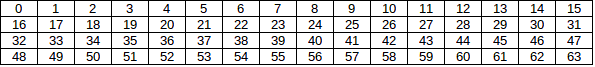
\includegraphics[scale=1]{figuras/fig101.png}
	\item Marque os múltiplos de 4.\\
	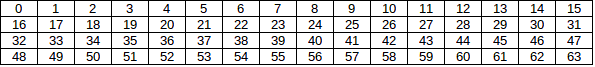
\includegraphics[scale=1]{figuras/fig101.png}
	\item Marque os múltiplos de 5.\\
	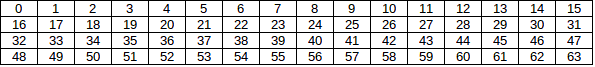
\includegraphics[scale=1]{figuras/fig101.png}
	\item Marque os múltiplos de 9.\\
	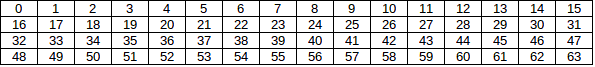
\includegraphics[scale=1]{figuras/fig101.png}
\end{enumerate}

\item Escreva certo ou errado.
\begin{enumerate}[a)]
\item O conjunto dos múltiplos de 7 é infinito.
\item O conjunto dos múltiplos de 5 é finito.
\item O conjunto dos múltiplos de 1 é unitário.
\item O menor múltiplo de qualquer número é zero.
\item O menor múltiplo de qualquer número é ele mesmo.
\item O conjunto  dos divisores de 12 é finito.
\item O conjunto dos divisores de 8 é infinito.
\item O conjunto dos divisores de 1 é unitário
\item O conjunto dos divisores de 7 é o vazio
\item O menor divisor de qualquer número é zero.
\item O menor divisor de qualquer número é 1.
\item O maior divisor de um número diferente de zero é ele mesmo.
\end{enumerate}

\item  Quais desses números são divisíveis por 2 ?
\begin{multicols}{5}
\begin{enumerate}[a)]
	\item 43
	\item 58
	\item 62
	\item 93
	\item 106
	\item 688
	\item 981
	\item 1000
	\item 3214
	\item 6847
	\item 14649
	\item 211116
	\item 240377
	\item 800001
	\item 647731350
\end{enumerate}
\end{multicols}

\item Quais desses números são divisíveis por 3?
\begin{multicols}{4}
\begin{enumerate}[a)]
	\item 72
	\item 83
	\item 58
	\item 96
	\item 123
	\item 431
	\item 583
	\item 609
	\item 1111
	\item 1375
	\item 1272
	\item 4932
	\item 251463
	\item 1040511
	\item 8000240
	\item 7112610
\end{enumerate}
\end{multicols}

\item Quais desses números são divisíveis por 4?
\begin{multicols}{4}
\begin{enumerate}[a)]
	\item 200
	\item 323
	\item 832
	\item 918
	\item 1020
	\item 3725
	\item 4636
	\item 7812
	\item 19012
	\item 24714
	\item 31433
	\item 58347
	\item 1520648
	\item 3408549
	\item 5331122
	\item 2000008
\end{enumerate}
\end{multicols}

\item Quais desses números são divisíveis por 5?
\begin{multicols}{4}
\begin{enumerate}[a)]
	\item 83
	\item 45
	\item 678
	\item 840
	\item 1720
	\item 1089
	\item 2643
	\item 4735
	\item 2643
	\item 8310
	\item 7642
	\item 12315
	\item 471185
	\item 648933
	\item 400040
	\item 3821665
\end{enumerate}
\end{multicols}

\item Quais destes números são divisíveis por 6?
\begin{multicols}{4}
\begin{enumerate}[a)]
	\item 126
	\item 452
	\item 831
	\item 942
	\item 1236
	\item 3450
	\item 2674
	\item 7116
	\item 10008
	\item 12144
	\item 12600 
	\item 51040
	\item 521125
	\item 110250
	\item 469101
	\item 4000002
\end{enumerate}
\end{multicols}

\item Quais desses números são divisíveis por 9?
\begin{multicols}{4}
\begin{enumerate}[a)]
	\item 504
	\item 720
	\item 428
	\item 818
	\item 3169
	\item 8856
	\item 4444
	\item 9108
	\item 29133
	\item 36199
	\item 72618
	\item 98793
	\item 591218
	\item 903402
	\item 174150
	\item 2000601
\end{enumerate}
\end{multicols}

\item Quais destes números são divisíveis por 10?
\begin{multicols}{4}
\begin{enumerate}[a)]
	\item 482
	\item 520
	\item 655
	\item 880
	\item 1670
	\item 1829
	\item 3687
	\item 8730
	\item 41110
	\item 29490
	\item 34002
	\item 78146
	\item 643280
	\item 128456
	\item 890005
	\item 492370
\end{enumerate}
\end{multicols}

\item determine:
\begin{multicols}{4}
\begin{enumerate}[a)]
	\item d(14);
	\item d(13);
	\item d(15);
	\item d(16).
\end{enumerate}
\end{multicols}

\item Efetue as divisões e responda:
\begin{multicols}{2}
\begin{enumerate}[a)]
	\item 495 é divisível por 9?
	\item 1260 é divisível por 7?
	\item 378 é divisível por 12?
	\item 14 é divisível por 182?
\end{enumerate}
\end{multicols}

\item Verifique se 182 é divisível por 7, por 8, por 11 e por 13.

\item Escreva:
\begin{multicols}{2}
\begin{enumerate}[a)]
	\item o número natural que só tem um divisor;
	\item um número natural que fica entre 20 e 30 e tem exatamente dois divisores;
	\item o número natural que tem infinitos divisores;
	\item um número natural que tem mais do que 8 divisores.
\end{enumerate}
\end{multicols}

\item Para descobrir os divisores de 8, há necessidade de dividir 8 por números naturais maiores do que ele? Responda e justifique.

\item Determine:
\begin{enumerate}[a)]
	\item os divisores comuns de 12 e 20, isto é, os números que são divisores de 12 e também são divisores de 20;
	\item os divisores comuns de 14 e 9.
\end{enumerate}

\item O mês de março possui 31 dias. Celso jogou tênis, neste  mês, nos dias ímpares e Rodrigo nos dias múltiplos de 3. Quantas vezes ambos jogaram tênis no mesmo dia? 

\item Quantos são os números primos até 30? Responda usando o crivo de Eratóstenes e a tabela abaixo.
\begin{center}
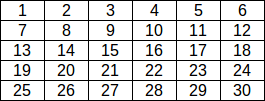
\includegraphics[scale=1]{figuras/fig102.png}
\end{center}

\item Quais são os números divisíveis por 6 entre 70 e 100 ?

\item Dados os números 39, 140, 245, 384, 720 e 2600, verifique os que são divisíveis por :
\begin{multicols}{2}
\begin{enumerate}[a)]
	\item 2
	\item 3
	\item 4
	\item 5
	\item 6
	\item 8
	\item 9
	\item 10
\end{enumerate}
\end{multicols}

\item Qual é o maior número de dois algarismos divisível por 5 ?

\item Qual é o menor número de três algarismos divisível por 3 ?

\item Um número é composto de três algarismos. O algarismo das unidades é 2 e o das centenas é 5. Determine os possíveis valores do algarismo das dezenas para que esse número seja divisível por 3.

\item Este é um jogo de números cruzados, parecido com as palavras cruzadas. Você deverá substituir os espaços por um algarismo, de modo que os números formados estejam de acordo com as seguintes instruções :

Horizontais :

A – Um número em que cada algarismo é o sucessor do algarismo anterior.\\
B – O maior número de três algarismos que seja divisível por 2.\\
C – Um número menor que 300.

Verticais :

A – Um número que não é divisível por 2.\\
B – Um número divisível por 3, mas não por 2.\\
C – Um número de três algarismos iguais.\\
\begin{center}
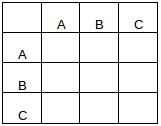
\includegraphics[scale=1]{figuras/fig103.png}
\end{center}
\end{list}